\documentclass[11pt]{book}
\usepackage{graphicx}
\usepackage{amsmath,amssymb}
\usepackage{amsthm}
\usepackage[hidelinks]{hyperref}
\usepackage{listings}
\usepackage{xcolor}
\usepackage{booktabs}

\lstset{basicstyle=\ttfamily\small, breaklines=true, frame=single,
        backgroundcolor=\color{gray!8}, showstringspaces=false}

\newenvironment{lesson}
  {\par\medskip\noindent\begin{minipage}{\linewidth}\itshape\textbf{Lesson.} }
  {\end{minipage}\medskip\par}

\theoremstyle{definition}
\newtheorem{example}{Example}[chapter]
\newtheorem{problem}{Problem}[chapter]
\newtheorem{keyresult}{Key result}[chapter]
\newenvironment{answer}
  {\par\smallskip\noindent\small\textbf{Answer.} }
  {\par\smallskip}

\title{The Vanguard Arm\\
  \large Theory, Decisions, and Lessons from a Mars Rover Manipulator\\
  \normalsize Project Vanguard --- BITS Pilani Hyderabad}
\author{Krithin Poola \and Claude (documentation \& reference)}
\date{Started July 2026 --- a living document}

\begin{document}
\maketitle
\tableofcontents

\part{The Build Journal}
\chapter{Why This Stack}
\label{ch:why}

This book documents the design, theory, and hard lessons of the Vanguard rover arm ---
manipulation autonomy for the BITS Pilani Hyderabad Mars Rover team, built to win IRC~2027 and
grow into a research platform. Every chapter is written in the same session the work happened,
so the reasoning here is what we actually thought, not a cleaned-up retrospective.

\section{The mission, worked backwards}

The arm exists to score points in four competitions (IRC, ARC, ERC, URC) whose manipulation
tasks --- studied from the primary rulebooks --- collapse into six reusable skills: grasp \&
carry, panel operations, connector insertion, oriented placement, sampling support, and
read-\&-report. IRC's IDMO panel (buttons, switches, knobs, a 3-pin plug), ARC's propellant
hose, ERC's RJ-45, and URC's board connectors are one skill family wearing four costumes. The
central architectural bet follows: \emph{build skills, not missions}. A new rulebook becomes a
re-orchestration, not a rebuild.

Two strategy decisions bound everything else:
\begin{enumerate}
  \item \textbf{Reliable assisted teleoperation wins IRC 2027; genuine autonomy is the ERC 2027
  goal.} Top teams win on reliability and operator skill. Autonomy is invested exactly where the
  rulebook prices it (IRC's RADO delivery: autonomous = 100\% of points, teleoperated = 50\%).
  \item \textbf{Simulation first.} The physical arm arrives months after work begins. The stack
  is therefore built against an Isaac Sim digital twin exposing \emph{identical ROS~2
  interfaces} to the future hardware --- so hardware arrival is an integration event, not a
  starting gun. This same twin later becomes the benchmark environment of our first paper.
\end{enumerate}

\section{One mental model}
\label{sec:mental-model}

A manipulator is a chain of rigid-body transforms in $SE(3)$, and every tool in the stack is
that one mathematical object viewed differently. The URDF \emph{declares} the chain. TF2
\emph{broadcasts} it. Forward kinematics \emph{composes} it:
\[
  T_{\text{ee}}(\theta) \;=\; e^{[\mathcal{S}_1]\theta_1} e^{[\mathcal{S}_2]\theta_2} \cdots
  e^{[\mathcal{S}_n]\theta_n}\, M ,
\]
the product of exponentials over the joint screw axes $\mathcal{S}_i$ acting on the home pose
$M$. Inverse kinematics \emph{inverts} it --- nonlinear, multi-solution, and ill-conditioned
near singularities. The Jacobian \emph{differentiates} it, $\mathcal{V} = J(\theta)\dot\theta$,
and is why teleop jogging, visual servoing, and singularity handling are the same problem.
MoveIt~2 \emph{plans} through the chain; \texttt{ros2\_control} \emph{executes} along it; Isaac
Sim \emph{simulates} it from the same URDF. Ten tools, one idea.

Two consequences we will meet repeatedly:
\begin{itemize}
  \item \textbf{Six degrees of freedom is the floor, not a luxury.} Connector insertion
  requires commanding an arbitrary approach \emph{orientation} at an arbitrary position ---
   six constraints. A 5-DoF arm can reach the socket but cannot, in general, present the plug
  square to it.
  \item \textbf{Singularity is a property of the map, not the motor.} At a straight elbow,
  $J$ loses rank; some Cartesian velocities become unreachable and naive IK commands explode.
  We damp (damped least squares) rather than pretend precision the hardware doesn't have.
\end{itemize}

\section{Infrastructure decisions (recorded before the first line of code)}
\label{sec:infra}

\begin{description}
  \item[Platform.] Ubuntu 22.04 + ROS~2 Humble for the IRC season; migration to Jazzy/24.04 is
  \emph{scheduled} (post-IRC window, Humble EOL May 2027) rather than improvised.
  \item[Containers.] Development happens in a devcontainer (\texttt{ros:humble-ros-base-jammy});
  the rover will run a lean L4T-based runtime image on the Jetson. Deployment is
  \texttt{git pull \&\& docker compose up}, not dependency archaeology at 7\,am in a field.
  \item[DDS.] CycloneDDS as the team RMW, \texttt{--network=host --ipc=host} on every container,
  one \texttt{ROS\_DOMAIN\_ID}. This dissolves the classic ``container can't discover the
  robot'' failure class before anyone hits it.
  \item[TensorRT engines are built on the device that runs them.] Engines are not portable
  artifacts; on-rover engine generation is a scripted first-boot step (a lesson inherited
  directly from the APEX project).
  \item[Bring-up is native; runtime is containerized.] When a motor doesn't enumerate you want
  \texttt{dmesg} with zero layers in between. Containers earn their keep once drivers are
  stable.
  \item[Compute.] Development and Isaac scenes on a 12\,GB RTX laptop; heavy training
  (GR00T-class fine-tunes, RL) as containerized batch jobs on the university HPC. The nightly
  simulation regression runs on the docked laptop.
\end{description}

\section{Mistakes log, opened early}
\label{sec:mistakes-ch1}

This section exists in every chapter. Failures are recorded with root causes because they are
the highest-density teaching material we produce.

\begin{lesson}
\textbf{The paste-boundary error (day one).} The very first typed file of the project ---
\texttt{.devcontainer/Dockerfile.dev} --- ended up containing the JSON of
\texttt{devcontainer.json} pasted below the Dockerfile instructions; the build would have died
on the first JSON line. Found in review before first build. Root cause: transcribing two
reference files in one editing pass without a file-boundary check. Rule adopted: after typing
from reference, \emph{verify each file builds/parses on its own} before moving to the next.
The same failure family (paste-indent) cost a debugging session on APEX in June 2026.
\end{lesson}

\chapter{The Stand-In Arm}
\label{ch:standin}

\section{Why a UR5e we don't own}

Phase 0 needs an arm months before mechanical delivers one. The first plan was a hand-written
placeholder xacro; Krithin counter-proposed adopting an existing, battle-tested description ---
and the counter-proposal won the review. The Universal Robots UR5e matches our envelope almost
exactly (850\,mm reach, 5\,kg payload $\approx$ the IRC cache spec), ships an official MoveIt
configuration and an official NVIDIA Isaac Sim asset, is the arm every ROS~2 tutorial assumes,
and is the reference target of the GELLO teleoperation design we intend to build. There is also
a research reason: our first paper's benchmark is more reproducible if its baseline arm is one
any lab can load.

The stand-in comes with guardrails so UR conveniences cannot hide problems our real arm will
have:
\begin{itemize}
  \item \textbf{Generic IK only} (KDL / TracIK / pick\_ik) --- never the UR-specific analytic
  solver. Mech's arm will not have the UR's near-ideal wrist geometry.
  \item \textbf{Skills address \texttt{tool0} and named planning groups}, never joint names.
  Swapping in the real URDF must be a configuration change, not a refactor.
  \item \textbf{Gates re-run on swap.} Every skill success-rate measured on the UR5e is
  re-measured on the real description the week it lands.
\end{itemize}

\section{The two-process architecture (what confused us, drawn once)}
\label{sec:two-process}

The first launch attempt produced no GUI and a confused operator. The reason is the most
important architectural fact in ROS~2 manipulation:

\begin{center}
\begin{tabular}{ccc}
\textbf{Terminal 1: the driver} & & \textbf{Terminal 2: the planner} \\
\texttt{ur\_control.launch.py} & & \texttt{ur\_moveit.launch.py} \\
\hline
\texttt{ros2\_control\_node} & $\xleftarrow{\;\text{FollowJointTrajectory action}\;}$ &
MoveIt \texttt{move\_group} \\
hardware interface (mock) & $\xrightarrow{\;\texttt{/joint\_states}\;}$ & RViz + MotionPlanning \\
controllers (JTC, broadcasters) & &
\end{tabular}
\end{center}

The driver \emph{owns the hardware} (here `mock\_components', later our CAN drivers on the
Jetson) and exposes controllers; MoveIt is merely a \emph{client} of the
\texttt{FollowJointTrajectory} action. They are separate processes speaking DDS --- which is
why they can run in one container, two containers, or a laptop and a rover 500\,m apart,
unchanged. On competition day this same diagram is the base station (planner/UI) and the rover
(driver); the fake-hardware flag is the only line that changes.

Working vocabulary pinned by this exercise: \texttt{controller\_manager} loads and activates
controllers against the hardware interface; \texttt{joint\_state\_broadcaster} publishes what
the encoders (here, simulated) report; \texttt{scaled\_joint\_trajectory\_controller} executes
time-parameterized joint trajectories. The ``No GUI?'' moment resolved itself the instant the
second process started --- the GUI was never missing, it simply hadn't been asked for.

\section{No gripper --- by design}
\label{sec:no-gripper}

The stock \texttt{ur\_description} ends at \texttt{tool0}, a bare flange: industrial arms ship
without end-effectors because the end-effector is application-specific. This mirrors our own
architecture decision (interface spec \S 5): the gripper is a \emph{swappable module} on a
standard flange, developed on its own track by mechanical. In simulation we will attach a
Robotiq 2F-85 description at \texttt{tool0} when grasping work begins --- it is the standard
research gripper, its ROS~2 description is public, and its parallel-jaw morphology matches what
mech is likely to build first. Until then, MoveIt plans to \texttt{tool0} poses, which is
exactly how the skills should address the arm anyway.

\section{Mistakes log}

\begin{lesson}
\textbf{Prescribing a launch file that doesn't exist (Claude's error).} The instruction said
\texttt{demo.launch.py}; Humble's \texttt{ur\_moveit\_config} ships \texttt{ur\_moveit.launch.py}
and expects a separately-launched driver. Root cause: quoting a newer distro's package layout
from memory instead of checking the installed package. Rule: before prescribing a launch,
verify it --- \texttt{ls \$(ros2 pkg prefix <pkg>)/share/<pkg>/launch/}. This check belongs in
the planned \texttt{ros2-debug} skill.
\end{lesson}

\begin{lesson}
\textbf{Ephemeral installs in \texttt{--rm} containers.} \texttt{ur\_robot\_driver} was
installed live inside a running container started with \texttt{--rm}; it will vanish with the
container. Anything installed interactively must be promoted to the Dockerfile the same day ---
the image is the single source of truth for the environment.
\end{lesson}

\begin{lesson}
\textbf{Placeholders are for replacing.} \texttt{docker exec -it <that-name> bash} was typed
verbatim, angle brackets and all. Trivial, universal, worth stating once: \texttt{< >} in any
command means ``substitute your value.'' Every teammate onboarding guide gets this sentence.
\end{lesson}

\begin{figure}[h]\centering
  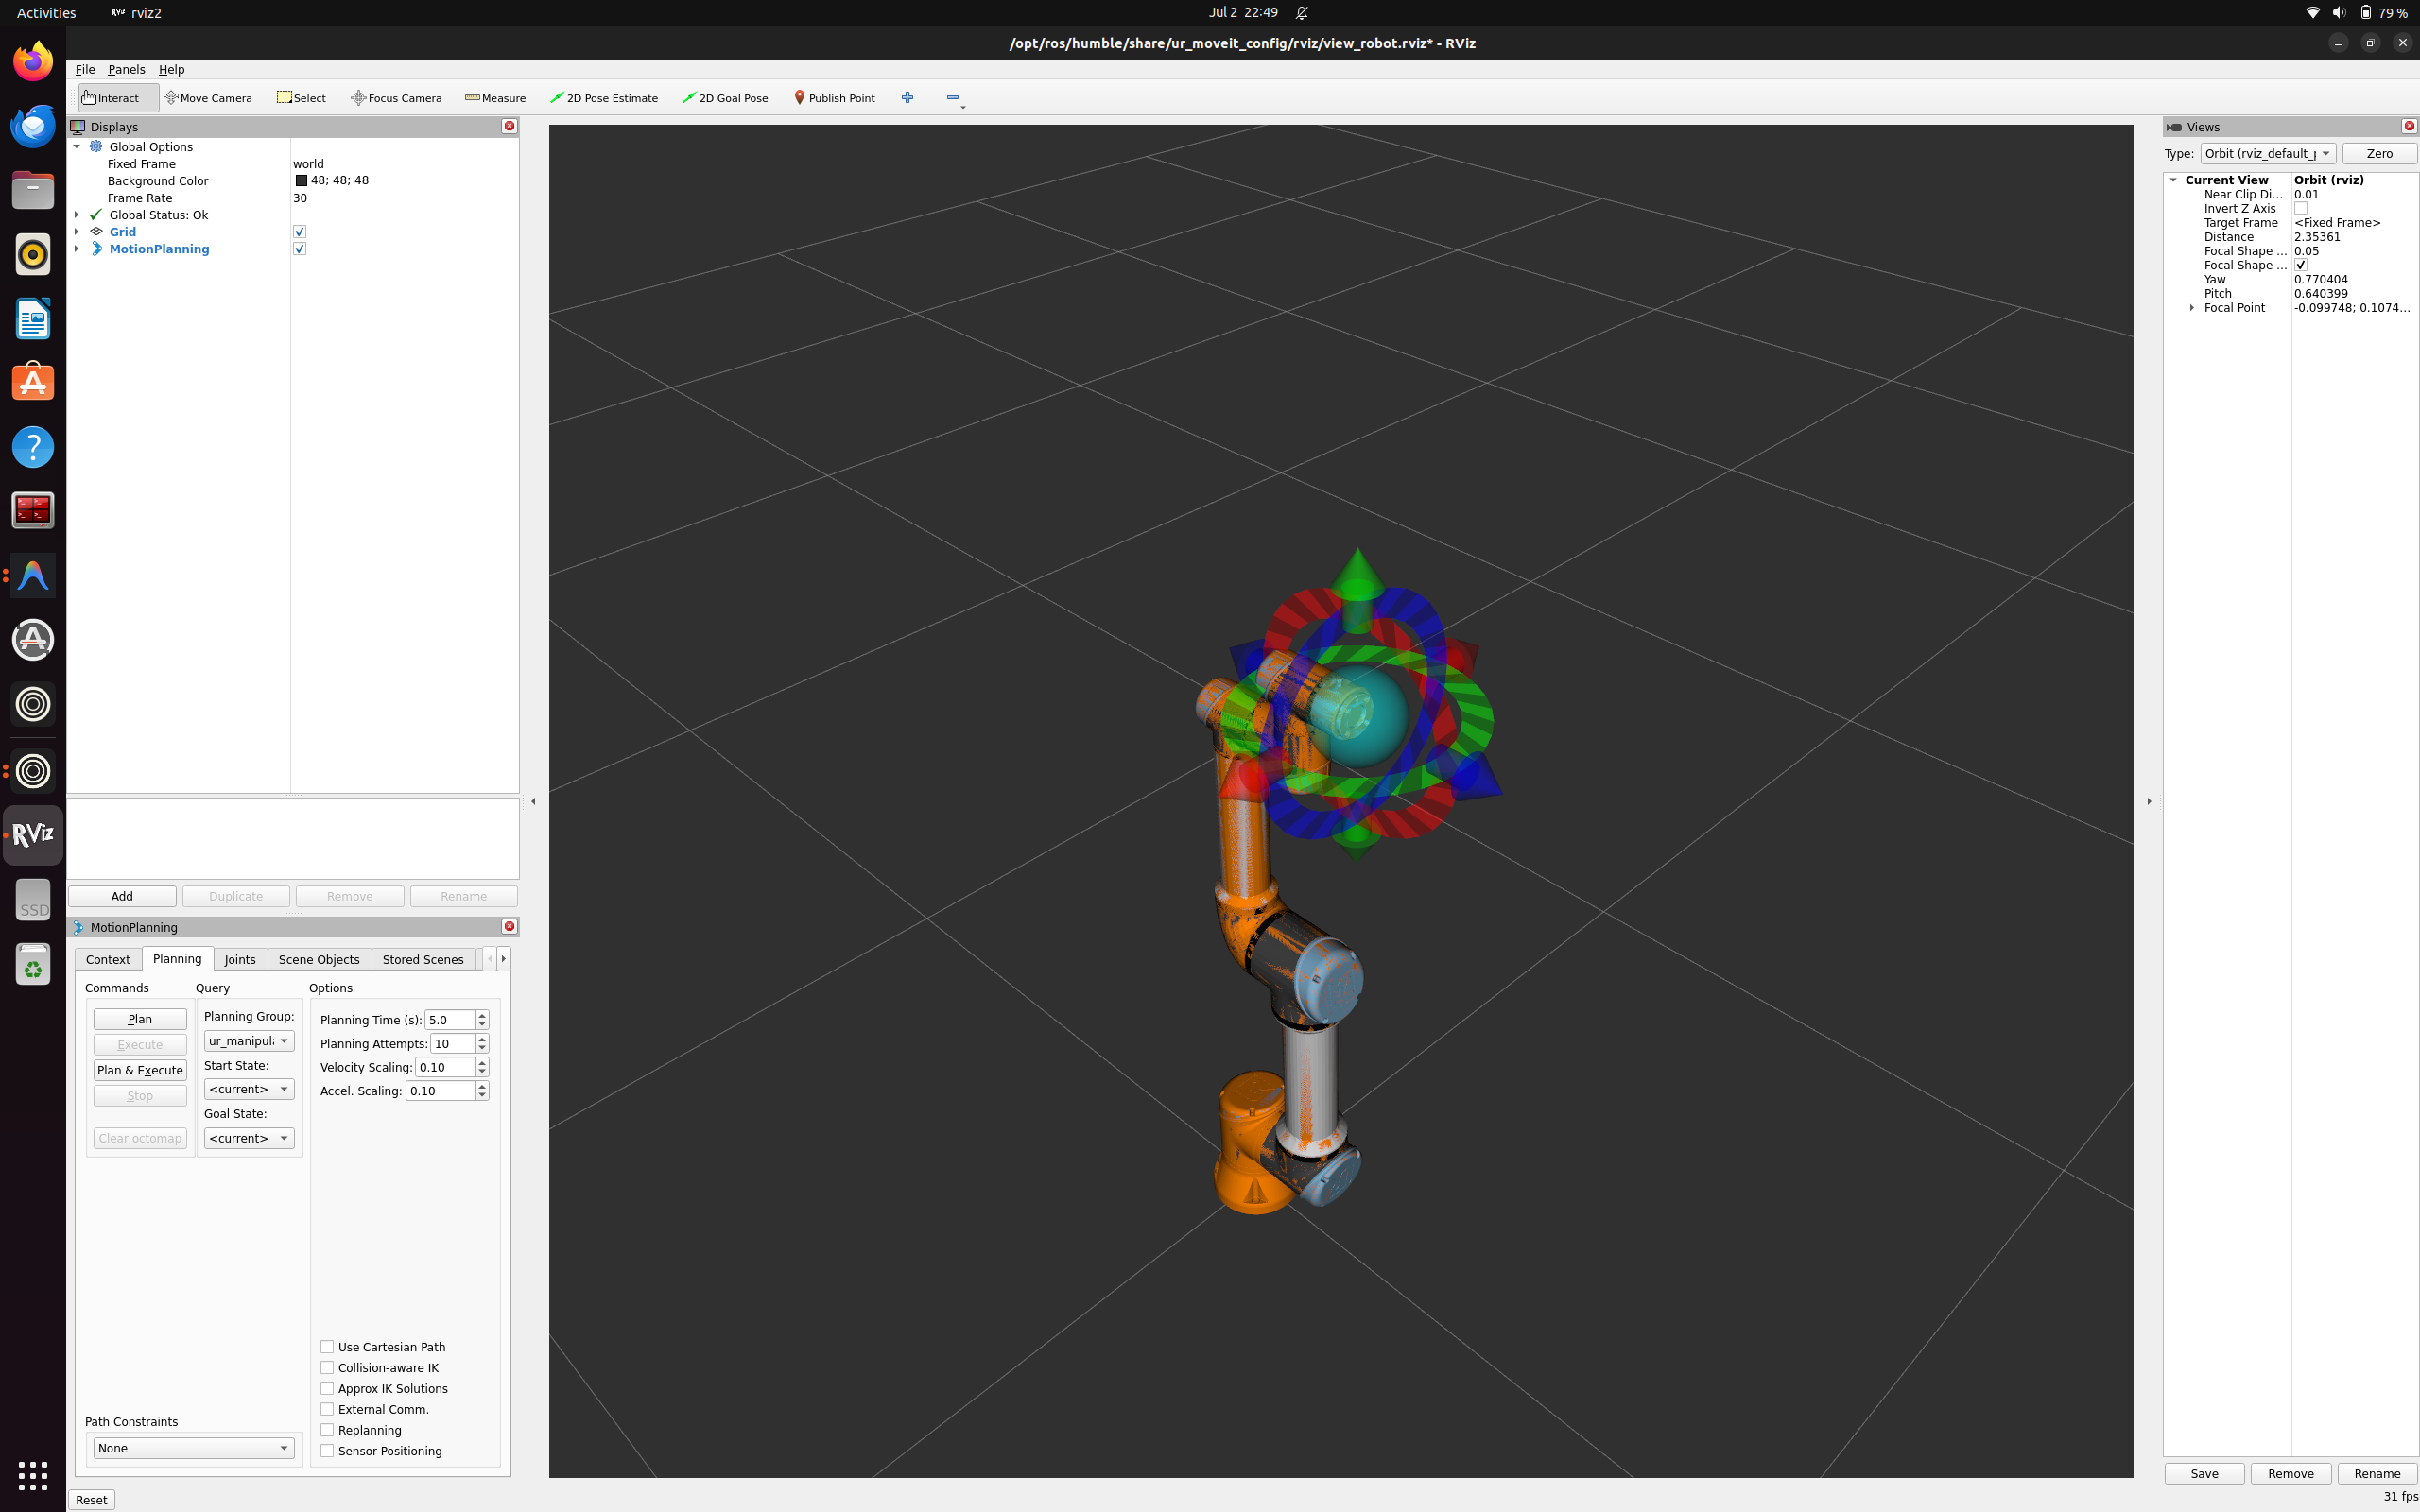
\includegraphics[width=0.9\linewidth]{figures/ch02_first_plan.png}
  \caption{First motion plan, 2 July 2026: UR5e on mock hardware inside the devcontainer.
  MoveIt's MotionPlanning panel with the \texttt{ur\_manipulator} group; the interactive
  marker (rings and sphere) sets the \texttt{tool0} goal pose. Velocity and acceleration
  scaling deliberately at 0.10 --- competition speed comes later, correctness comes first.}
  \label{fig:first-plan}
\end{figure}

\chapter{Speaking to Controllers}
\label{ch:controllers}

\section{The action interface every skill rides}

Chapter~\ref{ch:standin} established that MoveIt is just a client of the driver. This chapter
removes MoveIt from the loop: a 50-line \texttt{rclpy} node
(\texttt{ros2\_ws/src/scripts/send\_trajectory.py}) built a
\texttt{trajectory\_msgs/JointTrajectory} by hand and sent it to
\texttt{/scaled\_joint\_trajectory\_controller/follow\_joint\_trajectory} as a
\texttt{control\_msgs/action/FollowJointTrajectory} goal. The arm moved. That one exchange is
the load-bearing interface of the entire stack: every future skill --- grasp, panel-op,
insertion --- ultimately terminates in exactly this action call.

Anatomy of the message, as used:
\begin{itemize}
  \item \texttt{joint\_names} --- an \emph{ordered} list; position $i$ in every waypoint binds
  to name $i$. The controller maps names to its configured joints, so the order in the message
  is yours to choose --- but the positions must match \emph{your} chosen order exactly.
  \item \texttt{points[]} --- waypoints, each with \texttt{positions} and
  \texttt{time\_from\_start}. The controller spline-interpolates between them (Humble's JTC:
  `splines' method); you specify \emph{where} and \emph{when}, it decides the in-between.
  \item The action (not topic!) gives a goal/feedback/result contract: the client learns
  whether execution succeeded (\texttt{error\_code=0}) --- the primitive on which skill-level
  retry logic will be built.
\end{itemize}

Timing is the velocity command: the same two waypoints with \texttt{time\_from\_start} of
8\,s vs.\ 5\,s trace the same path at different speeds --- velocity is emergent
(\,$\Delta$position/$\Delta$time\,), not commanded. Competition pacing will be tuned exactly
here.

\section{Mistakes log}

\begin{lesson}
\textbf{Loud bug: wrong module.} \texttt{from trajectory\_msgs.action import ...} ---
\texttt{JointTrajectory} lives in \texttt{trajectory\_msgs.msg}. Instant \texttt{ImportError};
cost: seconds. Interface types live in \texttt{.msg}, action definitions in
\texttt{control\_msgs.action}; when unsure, \texttt{ros2 interface show <type>}.
\end{lesson}

\begin{lesson}
\textbf{Silent bug: a set where a list belongs.} \texttt{UR\_JOINTS} was typed with braces
\texttt{\{\}} --- a Python \emph{set}, which iterates in hash order. Since waypoint positions
bind to joint names \emph{by index}, a scrambled name order silently assigns the shoulder's
$-1.57$ to a wrist. In simulation, a curiosity; on hardware beside a panel, a collision. Two
rules adopted: (1) the future skills layer gets a trajectory sanity-checker (names, limits,
monotonic timing) in front of every action goal; (2) fail-loud beats fail-scrambled --- prefer
interfaces that reject wrong types over ones that reinterpret them.
\end{lesson}

\section{Experiment results (observed 2 July 2026, mock hardware)}

\paragraph{Timing.} With \texttt{p2} moved from $t{=}8$\,s to $t{=}5$\,s, the first leg
(start$\to$\texttt{p1}, 4\,s) was unchanged and the second leg ran in 1\,s instead of 4 ---
visibly $4\times$ faster over the identical path. Velocity was never commanded; it emerged
from waypoint spacing. (Observed exactly as predicted by the interpolation model above.)

\begin{figure}[h]\centering
  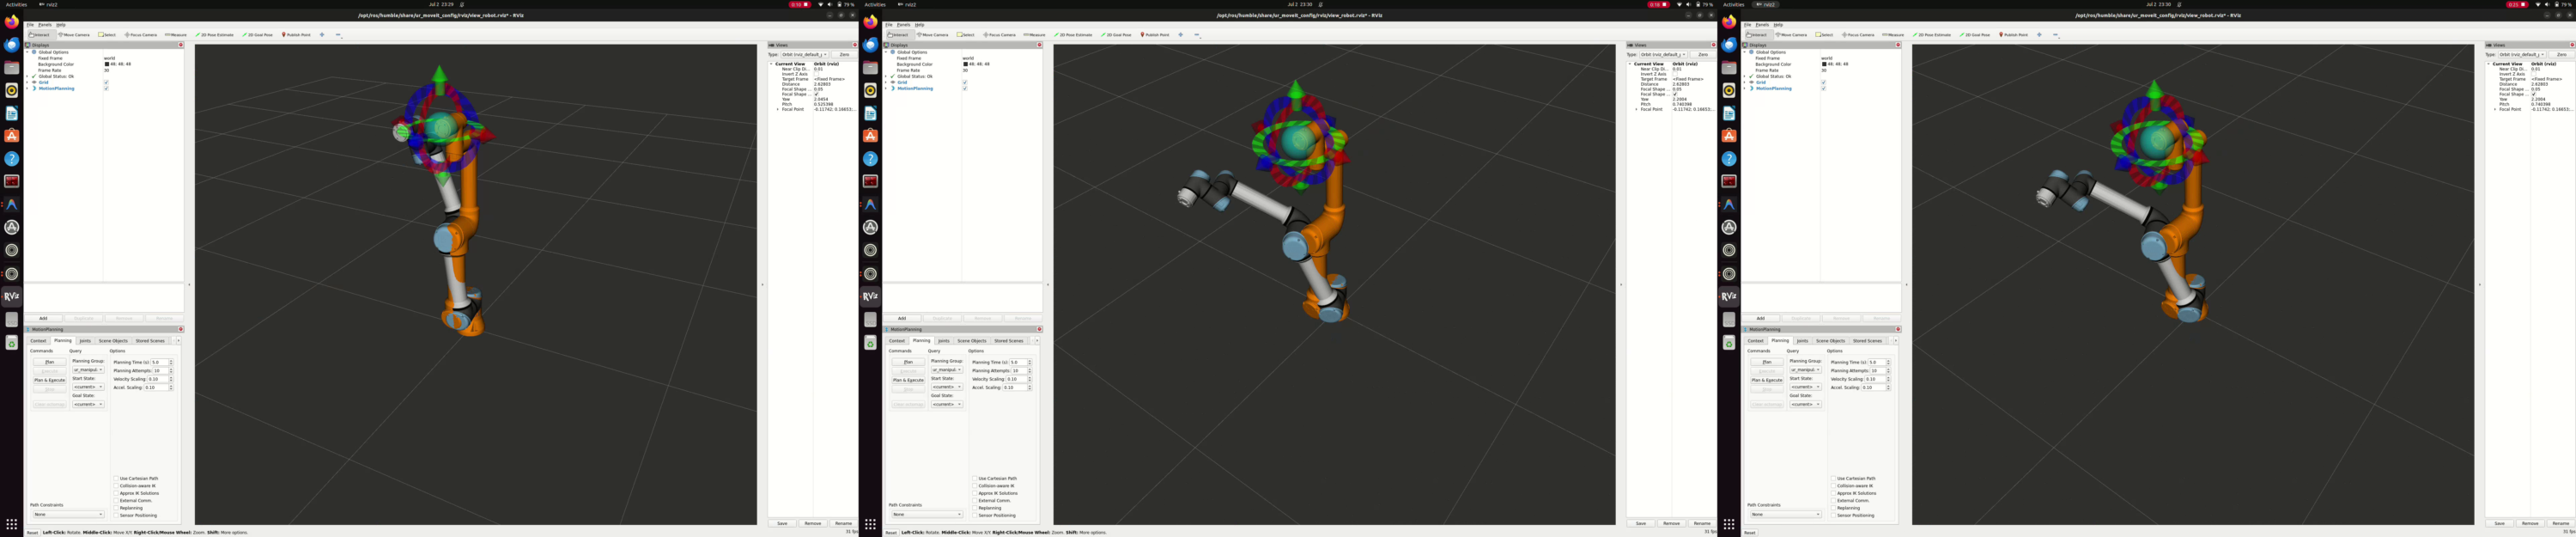
\includegraphics[width=\linewidth]{figures/ch03_trajectory_filmstrip.png}
  \caption{Frames from the screen recording of the two-waypoint trajectory executing in RViz
  --- the arm sweeping from home-ish through the elbow-bent midpoint to the target pose,
  commanded by \texttt{send\_trajectory.py} with no MoveIt in the loop.}
  \label{fig:filmstrip}
\end{figure}

\paragraph{The limit experiment: an impossible motion, executed.} Commanding the elbow to
$4.0$\,rad --- ${\sim}49^\circ$ past its $\pm\pi$ URDF limit --- produced neither a rejection
nor a clamp: \emph{the mock arm simply performed the impossible motion.} Three layers each
declined to protect us, and knowing which is which matters:
\begin{enumerate}
  \item \textbf{The trajectory controller} interpolates and forwards; Humble's JTC does not
  validate goals against URDF position limits.
  \item \textbf{Mock hardware} accepts any command --- that is what ``mock'' means.
  \item \textbf{MoveIt}, the layer that \emph{does} respect URDF limits when planning, was
  deliberately not in the loop --- our raw action client bypassed the only guard present.
\end{enumerate}
On the real UR, the vendor controller would have refused. On \emph{our} arm, there is no
vendor controller --- we are the vendor. Consequences adopted:
\begin{itemize}
  \item The Phase-1 hardware interface enforces joint limits (position, velocity, effort) in
  \texttt{read}/\texttt{write}, independent of anything upstream.
  \item The skills layer's trajectory sanity-checker (chapter's first lesson) gains a
  limits check --- names, limits, monotonic timing --- in front of \emph{every} action goal.
  \item Simulation passing is not evidence of safety when the simulation layer doesn't model
  the constraint. Know what each sim tier actually enforces (mock $<$ Isaac physics $<$
  hardware).
\end{itemize}


\part{Foundations --- Block A Theory}
\chapter{Rigid-Body Motion}
\label{ch:rigid}

Everything the arm does is described by rotations and translations of rigid bodies. This
chapter is the vocabulary; chapters~\ref{ch:fk} and \ref{ch:jac} are the grammar. Reference:
Modern Robotics ch.~3 (Lynch \& Park); read this chapter alongside it.

\section{Rotations}

A rotation matrix $R \in SO(3)$ is a $3\times3$ matrix satisfying
\[
  R^\top R = I, \qquad \det R = +1 .
\]
Its columns are the axes of the rotated frame expressed in the reference frame — that reading
solves most sign confusions. Rotations compose by multiplication and \emph{do not commute}:
rotating $90^\circ$ about $\hat z$ then $\hat x$ lands differently than $\hat x$ then $\hat z$.
Order is meaning: $R_{ab}R_{bc} = R_{ac}$ (subscript chains cancel like units).

\paragraph{Representations we will actually touch.}
\begin{itemize}
  \item \textbf{Rotation matrix} — what TF2 and all math uses internally; 9 numbers, 3 DoF.
  \item \textbf{Axis--angle} $(\hat\omega, \theta)$ — Rodrigues' formula reconstructs $R$:
  \begin{equation}
    R = I + \sin\theta\,[\hat\omega] + (1-\cos\theta)\,[\hat\omega]^2 ,
    \label{eq:rodrigues}
  \end{equation}
  where $[\hat\omega]$ is the skew-symmetric matrix of $\hat\omega$
  ($[\hat\omega]x = \hat\omega \times x$). This \emph{is} the exponential map:
  $R = e^{[\hat\omega]\theta}$.
  \item \textbf{Unit quaternion} $q = \big(\cos\tfrac\theta2,\; \hat\omega\sin\tfrac\theta2\big)$
  — 4 numbers, no singularities, what ROS messages carry (\texttt{x,y,z,w} order in
  \texttt{geometry\_msgs}, $w$ last — a classic bug source). $q$ and $-q$ are the same rotation
  (double cover).
  \item \textbf{Euler/RPY} — human-readable, gimbal-locked, used only at config-file boundaries
  (URDF \texttt{rpy=}). Never do math in RPY.
\end{itemize}

\begin{example}[Quaternion of a $90^\circ$ yaw]
$\hat\omega = (0,0,1)$, $\theta = \pi/2$:
$q = (\cos 45^\circ,\, 0,0,\sin 45^\circ) = (\tfrac{\sqrt2}{2}, 0, 0, \tfrac{\sqrt2}{2})$.
In ROS message order: $x{=}0,\, y{=}0,\, z{=}0.7071,\, w{=}0.7071$.
\end{example}

\section{Homogeneous transforms}

Pose = rotation + translation, packed as $T \in SE(3)$:
\[
  T = \begin{bmatrix} R & p \\ 0 & 1 \end{bmatrix}, \qquad
  T^{-1} = \begin{bmatrix} R^\top & -R^\top p \\ 0 & 1 \end{bmatrix} .
\]
Composition chains frames: $T_{ab}\,T_{bc} = T_{ac}$. This subscript-cancellation rule is the
whole of TF2: \texttt{lookup\_transform(a, c)} multiplies the chain of stored transforms for
you.

\begin{keyresult}
Never invert by transposing the whole $T$; only $R$ transposes. The translation picks up
$-R^\top p$.
\end{keyresult}

\begin{example}[Wrist camera to base]
The wrist camera sees an ArUco tag at $T_{\text{cam,tag}}$. The arm reports
$T_{\text{base,tool0}}$; hand--eye calibration gave $T_{\text{tool0,cam}}$. Where is the tag
for the planner?
\[
  T_{\text{base,tag}} \;=\; T_{\text{base,tool0}}\; T_{\text{tool0,cam}}\; T_{\text{cam,tag}} .
\]
Every panel-servicing skill begins with exactly this triple product. A $2$\,mm error in the
middle factor (calibration) shifts every tag estimate by $2$\,mm --- which is why
chapter~B1 (hand--eye) exists.
\end{example}

\section{Twists and screws (the 60-second version)}

Angular and linear velocity pack into a twist $\mathcal V = (\omega, v) \in \mathbb R^6$. A
unit screw axis $\mathcal S = (\hat\omega,\, v)$ with $v = -\hat\omega \times q$ (for a
revolute joint through point $q$) generalizes ``rotation about a line.'' Matrix exponentials of
screws produce rigid displacements: $T = e^{[\mathcal S]\theta}$. That single fact powers the
next chapter's forward kinematics. For deeper treatment: MR~ch.~3.3; for the Lie-group view,
Sol\`a et al.\ (arXiv:1812.01537) --- read it \emph{after} this clicks numerically.

\section{Problems}

\begin{problem}
Show that $R_z(90^\circ)R_x(90^\circ) \neq R_x(90^\circ)R_z(90^\circ)$ by tracking where the
unit vector $\hat x$ lands under each. (No matrices needed --- rotate a pen.)
\end{problem}
\begin{answer}
First ordering (apply $R_x$ first, then $R_z$... careful: in a fixed frame, the \emph{left}
matrix acts last): $R_z R_x$ sends $\hat x \to R_x \hat x = \hat x \to R_z \hat x = \hat y$.
The other ordering sends $\hat x \to \hat y \to$ (rotation about $\hat x$) $\to \hat z$.
$\hat y \neq \hat z$: non-commutative.
\end{answer}

\begin{problem}
Using \eqref{eq:rodrigues}, compute $R$ for $\hat\omega = (0,0,1)$, $\theta = 90^\circ$, and
verify it maps $\hat x \to \hat y$.
\end{problem}
\begin{answer}
$[\hat\omega] = \begin{bmatrix}0&-1&0\\1&0&0\\0&0&0\end{bmatrix}$, $\sin\theta = 1$,
$1-\cos\theta = 1$, $[\hat\omega]^2 = \mathrm{diag}(-1,-1,0)$. Sum:
$R = \begin{bmatrix}0&-1&0\\1&0&0\\0&0&1\end{bmatrix}$; first column $= \hat y$. \qedhere
\end{answer}

\begin{problem}
$T_{\text{base,tool0}}$ has $R = R_z(90^\circ)$ and $p = (0.4, 0.1, 0.5)$. Compute
$T^{-1}$ and state what frame relationship it represents.
\end{problem}
\begin{answer}
$R^\top = R_z(-90^\circ)$;
$-R^\top p = -R_z(-90^\circ)(0.4,0.1,0.5) = -(0.1, -0.4, 0.5) = (-0.1, 0.4, -0.5)$.
It is $T_{\text{tool0,base}}$: the base pose as seen from the tool.
\end{answer}

\begin{problem}[transfer]
Your teammate reports the gripper quaternion as $(0.7071, 0, 0, 0.7071)$ ``in ROS order.''
What are the two possible rotations they might mean, and how do you disambiguate?
\end{problem}
\begin{answer}
If $(x,y,z,w)$: $x = 0.7071, w = 0.7071$ → $90^\circ$ about $\hat x$. If they wrote $(w,x,y,z)$:
$90^\circ$ about $\hat z$. Disambiguate by convention-checking against a known pose (or just
\texttt{ros2 topic echo} and compare with RViz). Adopted team rule: always name the convention
when writing quaternions down.
\end{answer}

\chapter{Forward Kinematics: the Product of Exponentials}
\label{ch:fk}

Forward kinematics answers: \emph{given joint angles $\theta$, where is the tool?} The URDF
answers it numerically every time \texttt{robot\_state\_publisher} broadcasts TF; this chapter
is what that computation actually is. Reference: MR ch.~4.

\section{The formula}

Choose a home configuration (all $\theta_i = 0$) and record $M \in SE(3)$, the tool frame at
home. For each joint $i$, record its screw axis $\mathcal S_i$ (in the base frame, at home).
Then
\begin{equation}
  T_{\text{base,tool}}(\theta) \;=\;
  e^{[\mathcal S_1]\theta_1}\, e^{[\mathcal S_2]\theta_2} \cdots e^{[\mathcal S_n]\theta_n}\, M .
  \label{eq:poe}
\end{equation}
Each factor ``turns on'' one joint, in order from base to tip, then $M$ places the tool. For a
revolute joint through point $q_i$ with axis $\hat\omega_i$:
$\mathcal S_i = (\hat\omega_i,\; -\hat\omega_i \times q_i)$.

Why PoE and not Denavit--Hartenberg: no frame-assignment ritual, no four-parameter bookkeeping,
axes read straight off the CAD/URDF, and it composes cleanly with everything in
chapter~\ref{ch:rigid}. (DH still appears in older papers and UR's own documentation ---
recognize it, don't adopt it.)

\section{Worked example: the 2R planar arm}
\label{sec:2r}

Two links, lengths $l_1, l_2$, both joints about $\hat z$, arm along $\hat x$ at home.

\textbf{Setup.} $M = \begin{bmatrix} I & (l_1{+}l_2, 0, 0)^\top \\ 0 & 1\end{bmatrix}$;
$\mathcal S_1 = (0,0,1;\; 0,0,0)$ (axis through origin);
joint 2 passes through $q_2 = (l_1, 0, 0)$:
$v_2 = -\hat z \times q_2 = -(0, l_1, 0)$, so $\mathcal S_2 = (0,0,1;\; 0, -l_1, 0)$.

\textbf{Result} (expanding \eqref{eq:poe}, or by trigonometry):
\begin{equation}
  x = l_1\cos\theta_1 + l_2\cos(\theta_1{+}\theta_2), \qquad
  y = l_1\sin\theta_1 + l_2\sin(\theta_1{+}\theta_2) .
  \label{eq:2rfk}
\end{equation}

\textbf{Sanity limits} (always do these): $\theta = (0,0)$ gives $(l_1{+}l_2,\,0)$ — home.
$\theta = (0, 180^\circ)$ gives $(l_1 - l_2,\, 0)$ — folded back. $\theta = (90^\circ, 0)$
gives $(0,\, l_1{+}l_2)$ — straight up.

\begin{example}[Numbers]
$l_1 = l_2 = 1$, $\theta = (30^\circ, 45^\circ)$:
$x = \cos 30^\circ + \cos 75^\circ = 0.8660 + 0.2588 = 1.1248$;
$y = \sin 30^\circ + \sin 75^\circ = 0.5 + 0.9659 = 1.4659$.
\end{example}

\section{The UR5e through this lens}

The UR5e is six revolute joints; its screw axes come from the frame data in
\texttt{ur\_description} (the \texttt{\_kinematics.yaml} + xacro chain you met in
chapter~\ref{ch:standin}). Structurally: joint~1 yaws about the base $\hat z$; joints 2, 3, 4
pitch about parallel $\hat y$-axes (shoulder, elbow, wrist-1 — this parallel-axis triple is
why the arm has an elegant ``elbow-up/elbow-down'' geometry); joint 5 rolls; joint 6 pitches
the flange. When mech's arm arrives, our first analytical act will be writing ITS six screw
axes from the CAD --- the PoE table \emph{is} the kinematic datasheet.

\begin{keyresult}
The URDF is a serialized PoE model: each \texttt{<joint>}'s \texttt{<origin>} + \texttt{<axis>}
encode where $q_i$ and $\hat\omega_i$ sit relative to the parent. FK in
\texttt{robot\_state\_publisher}, planning in MoveIt, and physics in Isaac all consume this
one description --- which is why URDF correctness (chapter 2's guardrails, mech's CAD export)
is load-bearing for everything.
\end{keyresult}

\section{Problems}

\begin{problem}
For the 2R arm with $l_1 = 0.35$, $l_2 = 0.30$ (our interface-spec proportions), compute the
tool position at $\theta = (45^\circ, -30^\circ)$.
\end{problem}
\begin{answer}
$\theta_1{+}\theta_2 = 15^\circ$.
$x = 0.35\cos45^\circ + 0.30\cos15^\circ = 0.2475 + 0.2898 = 0.5373$;
$y = 0.35\sin45^\circ + 0.30\sin15^\circ = 0.2475 + 0.0776 = 0.3251$.
\end{answer}

\begin{problem}
Add a base yaw joint (about $\hat z$ at the origin, but now the 2R plane is vertical: joints
2, 3 about $\hat y$). Write the three screw axes $\mathcal S_1, \mathcal S_2, \mathcal S_3$ at
home (arm along $\hat x$).
\end{problem}
\begin{answer}
$\mathcal S_1 = (0,0,1;\,0,0,0)$;
$\mathcal S_2 = (0,1,0;\, -\hat y \times q_2)$ with $q_2 = 0 \Rightarrow v_2 = 0$ if the
shoulder sits at the origin, else $q_2=(0,0,h)$ gives $v_2 = -\hat y \times (0,0,h) = (-h,0,0)$;
$\mathcal S_3 = (0,1,0;\, -\hat y \times (l_1,0,h)) = (0,1,0;\; -h, 0, l_1)$.
(If you got $v_3 = (\!-h,0,l_1\!)$ check the cross-product order:
$\hat y \times (l_1,0,h) = (h,\,0,\,-l_1)$, negated $\Rightarrow (-h, 0, l_1)$.) \qedhere
\end{answer}

\begin{problem}
Why must the exponentials in \eqref{eq:poe} be multiplied in base-to-tip order? What physical
statement does swapping $e^{[\mathcal S_1]\theta_1}$ and $e^{[\mathcal S_2]\theta_2}$ make?
\end{problem}
\begin{answer}
Each screw is written in the \emph{home} base frame; turning joint 1 moves joint 2's axis
through space, and left-multiplication applies that displacement to everything downstream.
Swapping claims joint 2 rotates about its home axis regardless of joint 1 --- a different
(wrong) machine. Same reason matrix order mattered in Problem~1.1.
\end{answer}

\begin{problem}[bridge to practice]
In RViz you set the UR5e joints to all-zero with \texttt{joint\_state\_publisher\_gui}. The
arm points straight up, not along $\hat x$. What does that tell you about $M$ in
\texttt{ur\_description}, and why does it not matter for anything downstream?
\end{problem}
\begin{answer}
UR's home configuration has the arm vertical --- $M$ encodes that choice. PoE is indifferent:
$M$ is just ``where the tool is at zero.'' Conventions only need to be consistent between the
description and everything that consumes it --- which the URDF guarantees by construction.
\end{answer}

\chapter{Jacobians, Singularities, and Inverse Kinematics}
\label{ch:jac}

Chapter~\ref{ch:fk} maps joint angles to tool pose. This chapter differentiates that map ---
and inverts it. Teleop jogging, MoveIt's Cartesian goals, visual servoing (Block C), and the
straight-elbow experiment from chapter~\ref{ch:controllers} all live here. Reference: MR
ch.~5--6.

\section{The Jacobian}

Differentiating FK gives a linear map from joint velocities to tool twist:
\begin{equation}
  \mathcal V = J(\theta)\,\dot\theta, \qquad J \in \mathbb R^{6\times n}.
\end{equation}
Column $i$ answers: \emph{if only joint $i$ moves at unit speed, how does the tool move, at
this configuration?} For a revolute joint currently on axis $\hat\omega_i$ through point
$q_i$, with tool at $p$:
\[
  J_i = \begin{bmatrix} \hat\omega_i \\ \hat\omega_i \times (p - q_i) \end{bmatrix}.
\]
The linear part is lever-arm physics: velocity $=$ axis $\times$ arm. Long arm, fast tip ---
the same reason the shoulder joint dominates our reach envelope and the interface spec's
payload-at-extension clause exists.

\subsection{Worked example: the 2R Jacobian}

Differentiate \eqref{eq:2rfk} directly:
\begin{equation}
  J(\theta) = \begin{bmatrix}
    -l_1 s_1 - l_2 s_{12} & -l_2 s_{12} \\
     l_1 c_1 + l_2 c_{12} &  l_2 c_{12}
  \end{bmatrix},
  \qquad \det J = l_1 l_2 \sin\theta_2 .
  \label{eq:2rjac}
\end{equation}
($s_{12} = \sin(\theta_1{+}\theta_2)$, etc.)

\section{Singularities}

$\det J = l_1 l_2 \sin\theta_2$ vanishes at $\theta_2 = 0$ or $\pi$: the \textbf{straight (or
folded) elbow}. There the two columns become parallel --- both joints can only move the tip
\emph{perpendicular} to the arm; no joint motion produces velocity \emph{along} the arm.
Consequences, in increasing order of practical pain:
\begin{enumerate}
  \item A whole Cartesian direction is instantaneously unreachable.
  \item Near (not at) the singularity, reaching the ``hard'' direction requires enormous
  $\dot\theta$: $\dot\theta = J^{-1}v$ blows up as $\det J \to 0$.
  \item Numerical IK oscillates or explodes if implemented naively.
\end{enumerate}
The \textbf{manipulability} $w(\theta) = \sqrt{\det(JJ^\top)}$ ($= |l_1 l_2 \sin\theta_2|$ for
the 2R) measures distance from trouble; MoveIt Servo watches a version of this and scales
velocity down as $w$ shrinks --- that is the guard rail you will feel when jogging the UR5e
through a straight-arm pose.

\begin{keyresult}
Singularity is a property of the \emph{configuration}, not the target. The fix is never
``push harder'': it is damping (below), path shaping (approach panels with a bent elbow ---
operator playbook material), or redundancy (a 7th joint, which we don't have).
\end{keyresult}

\section{Inverse kinematics}

IK inverts FK: given desired $T_d$, find $\theta$. For our arms (and any arm without special
structure --- see chapter 2's generic-IK guardrail) this is numerical:

\textbf{Newton--Raphson:} iterate
$\;\theta \leftarrow \theta + J^{+}(\theta)\, e(\theta)\;$ where $e$ is the pose error (twist
from current to desired) and $J^+$ the pseudoinverse. Fast far from singularities; violent
near them.

\textbf{Damped least squares (DLS / Levenberg--Marquardt):}
\begin{equation}
  \Delta\theta = J^\top\!\left(JJ^\top + \lambda^2 I\right)^{-1} e .
  \label{eq:dls}
\end{equation}
The damping $\lambda$ trades tracking accuracy for bounded joint velocity: as $JJ^\top$ loses
rank, $\lambda^2 I$ keeps the inverse finite, so near-singular configurations produce slow,
sane motion instead of a joint-speed spike. This is the ``we damp rather than pretend
precision'' line from chapter 1, now with its formula. TracIK / KDL / pick\_ik are
production-grade wrappers around exactly this idea plus restarts and limits handling.

\subsection{Worked example: one NR step, by hand}

2R arm, $l_1 = l_2 = 1$, at $\theta = (0^\circ, 90^\circ)$, tool at $(1, 1)$ by
\eqref{eq:2rfk}. Target: $(1.2,\, 1.0)$, so $e = (0.2,\, 0)$.

From \eqref{eq:2rjac} with $s_1{=}0, c_1{=}1, s_{12}{=}1, c_{12}{=}0$:
\[
  J = \begin{bmatrix} -1 & -1 \\ 1 & 0 \end{bmatrix}, \quad \det J = 1, \quad
  J^{-1} = \begin{bmatrix} 0 & 1 \\ -1 & -1 \end{bmatrix}, \quad
  \Delta\theta = J^{-1} e = (0,\; -0.2)\ \text{rad}.
\]
New $\theta = (0^\circ,\, 78.54^\circ)$; FK gives $(1.199,\, 0.980)$. The $x$-error is nearly
closed in one step; $y$ picked up a small error because the step is first-order --- iteration
exists precisely to mop that up. Two or three more steps converge to sub-millimeter.

\section{Problems}

\begin{problem}
For the 2R arm at $\theta = (30^\circ, 0^\circ)$ (straight arm), compute $J$ and exhibit a
Cartesian velocity no $\dot\theta$ can produce.
\end{problem}
\begin{answer}
$s_{12}=s_1=\tfrac12$, $c_{12}=c_1=\tfrac{\sqrt3}2$:
$J = \begin{bmatrix} -\tfrac12 - \tfrac12 & -\tfrac12 \\ \tfrac{\sqrt3}2 + \tfrac{\sqrt3}2 &
\tfrac{\sqrt3}2\end{bmatrix}
   = \begin{bmatrix} -1 & -\tfrac12 \\ \sqrt3 & \tfrac{\sqrt3}2 \end{bmatrix}$;
columns are parallel (second $=$ first $\times \tfrac12$), $\det J = 0$. Both columns point
perpendicular to the arm direction $(\cos30^\circ, \sin30^\circ)$; any velocity \emph{along}
the arm, e.g.\ $v = (\cos30^\circ, \sin30^\circ)$, is unreachable.
\end{answer}

\begin{problem}
In the NR worked example, redo the step with DLS \eqref{eq:dls} and $\lambda = 0.5$. Compare
$\|\Delta\theta\|$ with the undamped step and explain the difference in one sentence.
\end{problem}
\begin{answer}
$JJ^\top = \begin{bmatrix} 2 & -1 \\ -1 & 1\end{bmatrix}$;
$JJ^\top + 0.25 I = \begin{bmatrix} 2.25 & -1 \\ -1 & 1.25\end{bmatrix}$, inverse
$= \tfrac{1}{1.8125}\begin{bmatrix}1.25 & 1 \\ 1 & 2.25\end{bmatrix}$. Then
$(JJ^\top{+}\lambda^2I)^{-1}e = \tfrac{1}{1.8125}(0.25,\, 0.2) = (0.1379, 0.1103)$ and
$\Delta\theta = J^\top(\cdot) = (-0.1379{+}0.1103,\; -0.1379) = (-0.0276,\, -0.1379)$.
$\|\Delta\theta\| = 0.141$ vs.\ $0.2$ undamped: damping shrinks (and slightly rotates) the
step, buying bounded velocity at the cost of extra iterations.
\end{answer}

\begin{problem}
The UR5e refused to jog smoothly through a fully-extended pose in MoveIt Servo (you will try
this). Which mechanism from this chapter is acting, and what are the operator's two escapes?
\end{problem}
\begin{answer}
Servo's singularity scaling: manipulability collapsed at full extension, so it throttles
Cartesian velocity toward zero. Escapes: re-approach along a direction the arm \emph{can}
move (perpendicular), or jog in joint space through the singular region and resume Cartesian
control on the far side. Playbook rule: plan panel approaches with a bent elbow.
\end{answer}

\begin{problem}[looking ahead to Block C]
Visual servoing will command tool velocities from image error: $v = -\kappa\, L^{+} e_{img}$.
Trace the full chain from a pixel error to motor current using the objects defined in
chapters~\ref{ch:rigid}--\ref{ch:jac} and the interfaces from chapter~\ref{ch:controllers}.
\end{problem}
\begin{answer}
Pixel error $\to$ interaction matrix $L^+$ $\to$ desired camera twist $\to$ (adjoint/frame
transform, ch.~\ref{ch:rigid}) tool twist $\mathcal V$ $\to$ DLS inverse of $J$
(ch.~\ref{ch:jac}) $\to$ $\dot\theta$ $\to$ velocity/position commands to the controller
(ch.~\ref{ch:controllers}) $\to$ driver $\to$ current. Every box is now named; Block C fills
in $L$.
\end{answer}


\end{document}
